\documentclass[a4paper]{article}

\usepackage[english]{babel}
\usepackage[utf8]{inputenc}
\usepackage[titletoc, toc]{appendix}
\usepackage{amsmath}
\usepackage{amsfonts}
\usepackage{graphicx}
\usepackage{mdframed}
\usepackage{cancel}
\usepackage{caption}
\usepackage{lipsum}
\usepackage{listings}
\usepackage{float}
\usepackage[colorinlistoftodos]{todonotes}

\title{Uncertainty Quantification (ACM41000) \\ Assignemt 3}

\author{Ian Towey \\ \\ 04128591}

\date{\today}

\lstdefinestyle{custom_py_style}{
  belowcaptionskip=1\baselineskip,
  breaklines=true,
  frame=L,
  xleftmargin=\parindent,
  language=Python,
  showstringspaces=false,
  basicstyle=\footnotesize\ttfamily,
  keywordstyle=\bfseries\color{green!40!black},
  commentstyle=\itshape\color{purple!40!black},
  identifierstyle=\color{blue},
  stringstyle=\color{orange}
}

% Number the subsubsections and include them in the TOC
\setcounter{secnumdepth}{3}
\setcounter{tocdepth}{3}
% \setcounter{section}{-1}

% Partial derivative
\newcommand*{\pd}[3][]{\ensuremath{\frac{\partial^{#1} #2}{\partial #3}}}

\newenvironment{aside}
  {\begin{mdframed}[style=0,%
      leftline=false,rightline=false,leftmargin=2em,rightmargin=2em,%
          innerleftmargin=0pt,innerrightmargin=0pt,linewidth=0.5pt,%
      skipabove=7pt,skipbelow=7pt]\footnotesize}
  {\end{mdframed}}

\begin{document}

  \maketitle

\tableofcontents
\newpage

\section{ODE with constant coefficients}
\subsection{Estimate $\alpha_{0}$ and $\alpha_{1}$ and $95\%$CI}

Estimate of differetial equation parameters

\begin{align*}
  \alpha_{0} &= 0.3290305 \\
  \alpha_{1} &= 0.1203271
\end{align*}


With 95\% confidence intervals

\begin{align*}
  0.3268669 < \alpha_{0} &< 0.3311941 \\
  0.1188871 < \alpha_{1} &< 0.1217670 
\end{align*}

\subsection{Estimate $\hat{f}$ and $95\%$CI}
$\hat{f}$ estimates and 95\% CI can be seen in Figure \ref{fig:density}
\subsection{Accuracy of fit analysis}

The $SSE = 0.001773525$, this is close to zero so the model should have a small random error somponent, this makes the model more useful for predictive purposes. \\ \\

The $ISE = 0.000002091086e$ is also very small with indictes the curve fits the unknown density $f$ very well. 

\subsection{Model comparison}
\begin{itemize}
 \item Nelson-Siegel soultion fits the majority of the data well, but does not fit the data less than 5 years very well(Figure \ref{fig:NelsonSeigel})	
 \item Svensson solution almost seems to interpolate the data and fits very well, but the resulting curve does not seem to be continous with discontinuities at the second and third data point(Figure \ref{fig:Svensson})
 \item Data2LD model fits the data well and is better than the Nelson-Siegel model fitting the points less than 5 years, but not as well as Svensson(Figure \ref{fig:data2ld})
\end{itemize}

\section{Two ODE models one with estimated forcing function and one time-varing parameter}

\section{Dynamical Systems}
Error :: singular matrix running Data2LD line 103 Q3.R

% \begin{appendix}
%    \newpage
%   \begin{figure}[H]
%     \centering
%     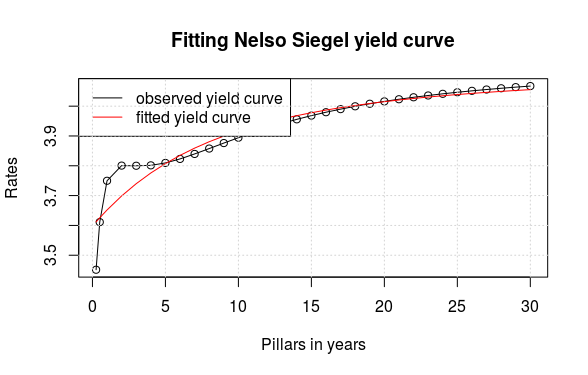
\includegraphics[width=1\textwidth]{NelsonSeigel.png}
%     \caption{\label{fig:NelsonSeigel}Nelson Seigel}
%   \end{figure}
%   
%   \begin{figure}[H]
%     \centering
%     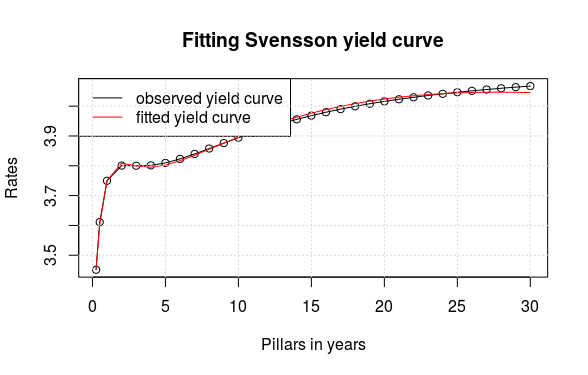
\includegraphics[width=1\textwidth]{svensson.png}
%     \caption{\label{fig:Svensson}Svensson.png}
%   \end{figure}
% 
%    \begin{figure}[H]
%       \centering
%       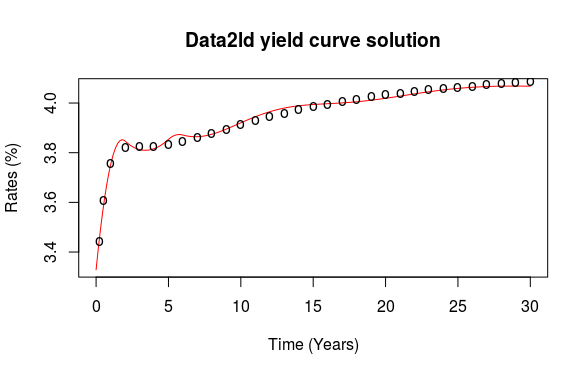
\includegraphics[width=1\textwidth]{data2ld.png}
%       \caption{\label{fig:data2ld}Data2ld}
%   \end{figure}
% 
%    \begin{figure}[H]
%       \centering
%       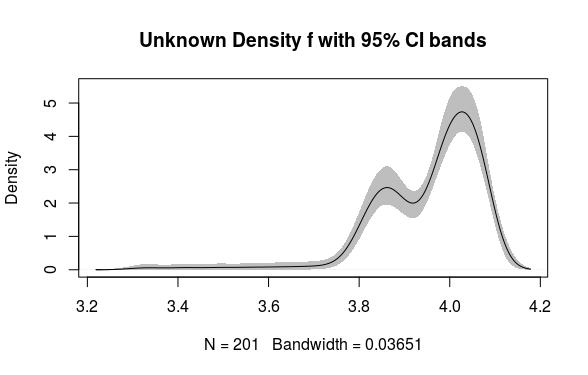
\includegraphics[width=1\textwidth]{density.png}
%       \caption{\label{fig:density}Density}
%   \end{figure}
%   
% 1   \sloppy
%     \newpage
%     \section{Q1 Code}
%    \lstinputlisting[language=R,style=custom_py_style]{/home/ian/Desktop/ACM41000-Uncertainty-Quantification/assignement3/Q1.R}
%     \newpage
%     \section{Q2 Code}
%    \lstinputlisting[language=R,style=custom_py_style]{/home/ian/Desktop/ACM41000-Uncertainty-Quantification/assignement3/Q2.R}
%     \newpage
%     \section{Q3 Code}
%    \lstinputlisting[language=R,style=custom_py_style]{/home/ian/Desktop/ACM41000-Uncertainty-Quantification/assignement3/Q3.R}
% \end{appendix}


\end{document}
